% Generated by tools/paper/render.py from main_text.py; edit the source there, not this file.
\begin{figure}[t]
\centering
\resizebox{\linewidth}{!}{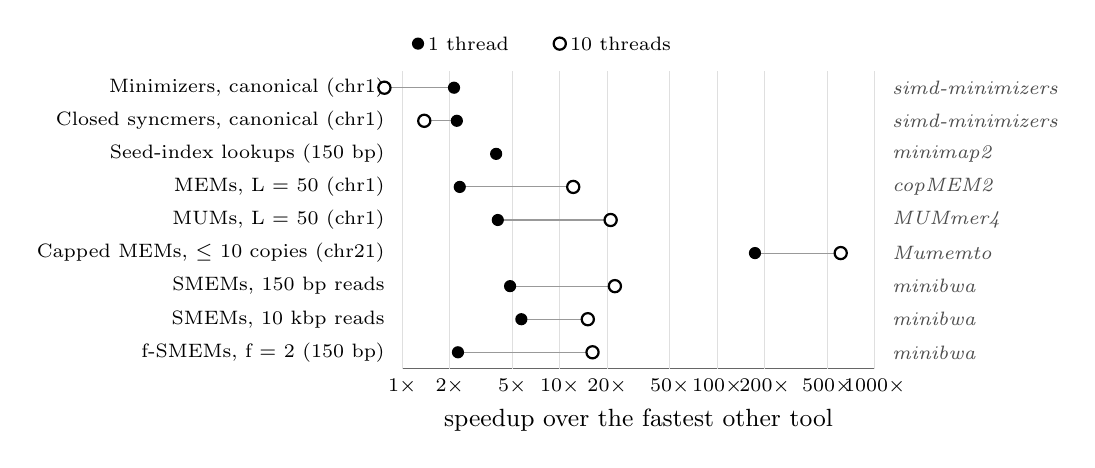
\begin{tikzpicture}
\draw[black!60] (0,0) -- (6.0,0);
\draw[gray!25] (0.000,0) -- (0.000,3.780);\node[below, font=\scriptsize] at (0.000,0) {1$\times$};
\draw[gray!25] (0.602,0) -- (0.602,3.780);\node[below, font=\scriptsize] at (0.602,0) {2$\times$};
\draw[gray!25] (1.398,0) -- (1.398,3.780);\node[below, font=\scriptsize] at (1.398,0) {5$\times$};
\draw[gray!25] (2.000,0) -- (2.000,3.780);\node[below, font=\scriptsize] at (2.000,0) {10$\times$};
\draw[gray!25] (2.602,0) -- (2.602,3.780);\node[below, font=\scriptsize] at (2.602,0) {20$\times$};
\draw[gray!25] (3.398,0) -- (3.398,3.780);\node[below, font=\scriptsize] at (3.398,0) {50$\times$};
\draw[gray!25] (4.000,0) -- (4.000,3.780);\node[below, font=\scriptsize] at (4.000,0) {100$\times$};
\draw[gray!25] (4.602,0) -- (4.602,3.780);\node[below, font=\scriptsize] at (4.602,0) {200$\times$};
\draw[gray!25] (5.398,0) -- (5.398,3.780);\node[below, font=\scriptsize] at (5.398,0) {500$\times$};
\draw[gray!25] (6.000,0) -- (6.000,3.780);\node[below, font=\scriptsize] at (6.000,0) {1000$\times$};
\node[font=\small] at (3.00,-0.65) {speedup over the fastest other tool};
\node[anchor=east, font=\scriptsize] at (-0.10,3.570) {Minimizers, canonical (chr1)};
\node[anchor=west, font=\scriptsize\itshape, black!70] at (6.10,3.570) {simd-minimizers};
\draw[black!40] (-0.227,3.570) -- (0.657,3.570);
\fill[black] (0.657,3.570) circle (2.2pt);
\draw[black, fill=white, thick] (-0.227,3.570) circle (2.2pt);
\node[anchor=east, font=\scriptsize] at (-0.10,3.150) {Closed syncmers, canonical (chr1)};
\node[anchor=west, font=\scriptsize\itshape, black!70] at (6.10,3.150) {simd-minimizers};
\draw[black!40] (0.279,3.150) -- (0.693,3.150);
\fill[black] (0.693,3.150) circle (2.2pt);
\draw[black, fill=white, thick] (0.279,3.150) circle (2.2pt);
\node[anchor=east, font=\scriptsize] at (-0.10,2.730) {Seed-index lookups (150 bp)};
\node[anchor=west, font=\scriptsize\itshape, black!70] at (6.10,2.730) {minimap2};
\fill[black] (1.192,2.730) circle (2.2pt);
\node[anchor=east, font=\scriptsize] at (-0.10,2.310) {MEMs, L = 50 (chr1)};
\node[anchor=west, font=\scriptsize\itshape, black!70] at (6.10,2.310) {copMEM2};
\draw[black!40] (0.730,2.310) -- (2.171,2.310);
\fill[black] (0.730,2.310) circle (2.2pt);
\draw[black, fill=white, thick] (2.171,2.310) circle (2.2pt);
\node[anchor=east, font=\scriptsize] at (-0.10,1.890) {MUMs, L = 50 (chr1)};
\node[anchor=west, font=\scriptsize\itshape, black!70] at (6.10,1.890) {MUMmer4};
\draw[black!40] (1.213,1.890) -- (2.646,1.890);
\fill[black] (1.213,1.890) circle (2.2pt);
\draw[black, fill=white, thick] (2.646,1.890) circle (2.2pt);
\node[anchor=east, font=\scriptsize] at (-0.10,1.470) {Capped MEMs, $\le$ 10 copies (chr21)};
\node[anchor=west, font=\scriptsize\itshape, black!70] at (6.10,1.470) {Mumemto};
\draw[black!40] (4.479,1.470) -- (5.568,1.470);
\fill[black] (4.479,1.470) circle (2.2pt);
\draw[black, fill=white, thick] (5.568,1.470) circle (2.2pt);
\node[anchor=east, font=\scriptsize] at (-0.10,1.050) {SMEMs, 150 bp reads};
\node[anchor=west, font=\scriptsize\itshape, black!70] at (6.10,1.050) {minibwa};
\draw[black!40] (1.369,1.050) -- (2.700,1.050);
\fill[black] (1.369,1.050) circle (2.2pt);
\draw[black, fill=white, thick] (2.700,1.050) circle (2.2pt);
\node[anchor=east, font=\scriptsize] at (-0.10,0.630) {SMEMs, 10 kbp reads};
\node[anchor=west, font=\scriptsize\itshape, black!70] at (6.10,0.630) {minibwa};
\draw[black!40] (1.512,0.630) -- (2.356,0.630);
\fill[black] (1.512,0.630) circle (2.2pt);
\draw[black, fill=white, thick] (2.356,0.630) circle (2.2pt);
\node[anchor=east, font=\scriptsize] at (-0.10,0.210) {f-SMEMs, f = 2 (150 bp)};
\node[anchor=west, font=\scriptsize\itshape, black!70] at (6.10,0.210) {minibwa};
\draw[black!40] (0.707,0.210) -- (2.416,0.210);
\fill[black] (0.707,0.210) circle (2.2pt);
\draw[black, fill=white, thick] (2.416,0.210) circle (2.2pt);
\fill[black] (0.2,4.130) circle (2.2pt) node[right, font=\scriptsize] {1 thread};\draw[black, fill=white, thick] (2.0,4.130) circle (2.2pt) node[right, font=\scriptsize] {10 threads};
\end{tikzpicture}}
\caption{Speedup of sporos over the fastest other tool for each task, on one thread (filled) and ten (hollow), each tool at its best on that many threads; the other tool is named on the right (Tables 1 to 5). copMEM2, MUMmer4, minibwa, bwa fastmap and Mumemto use one thread; the seed-lookup harnesses run one.}\label{fig:speedups}
\end{figure}
